\section{Schéma électrique}
Voici les schémas électrique de nôtre montage :

\begin{figure}[H]
    \centering
    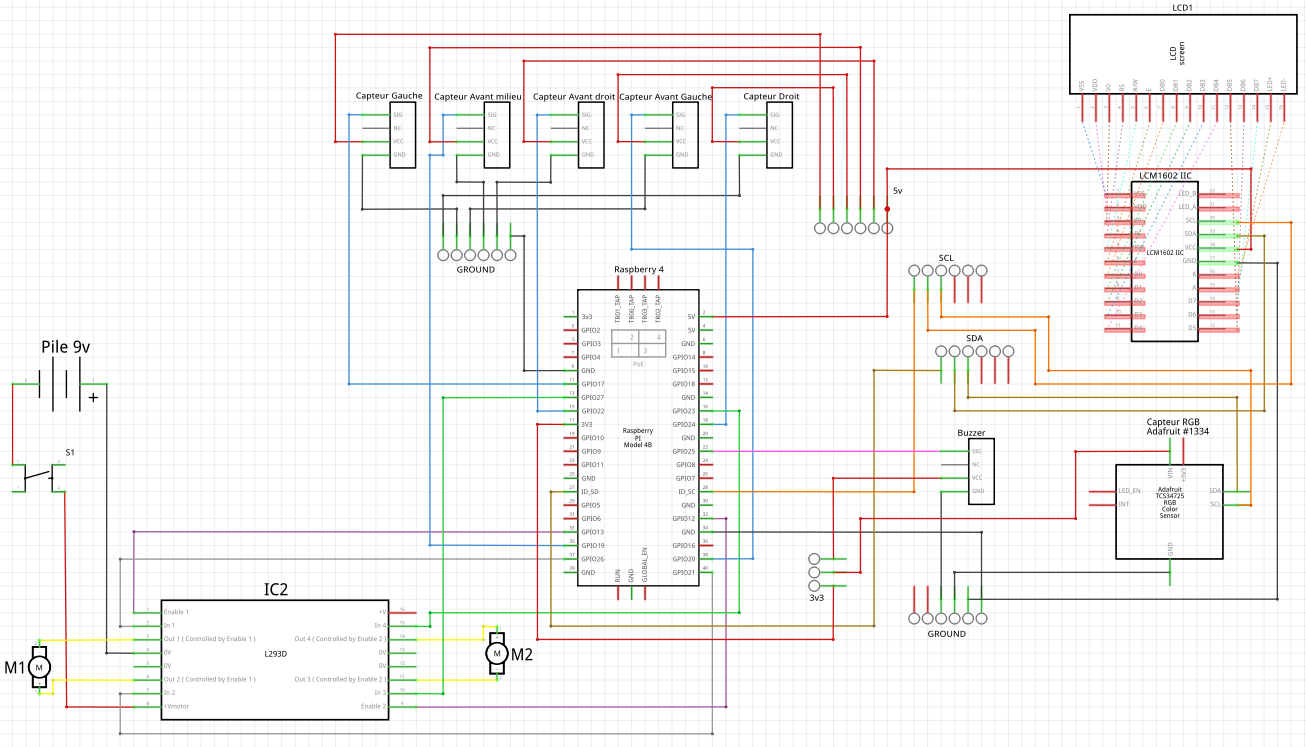
\includegraphics[width=1.0\textwidth]{image/shema_elec.png}
    \caption{Schéma de notre montage électrique}
    \label{fig:capteurs}
\end{figure}

\begin{figure}[H]
    \centering
    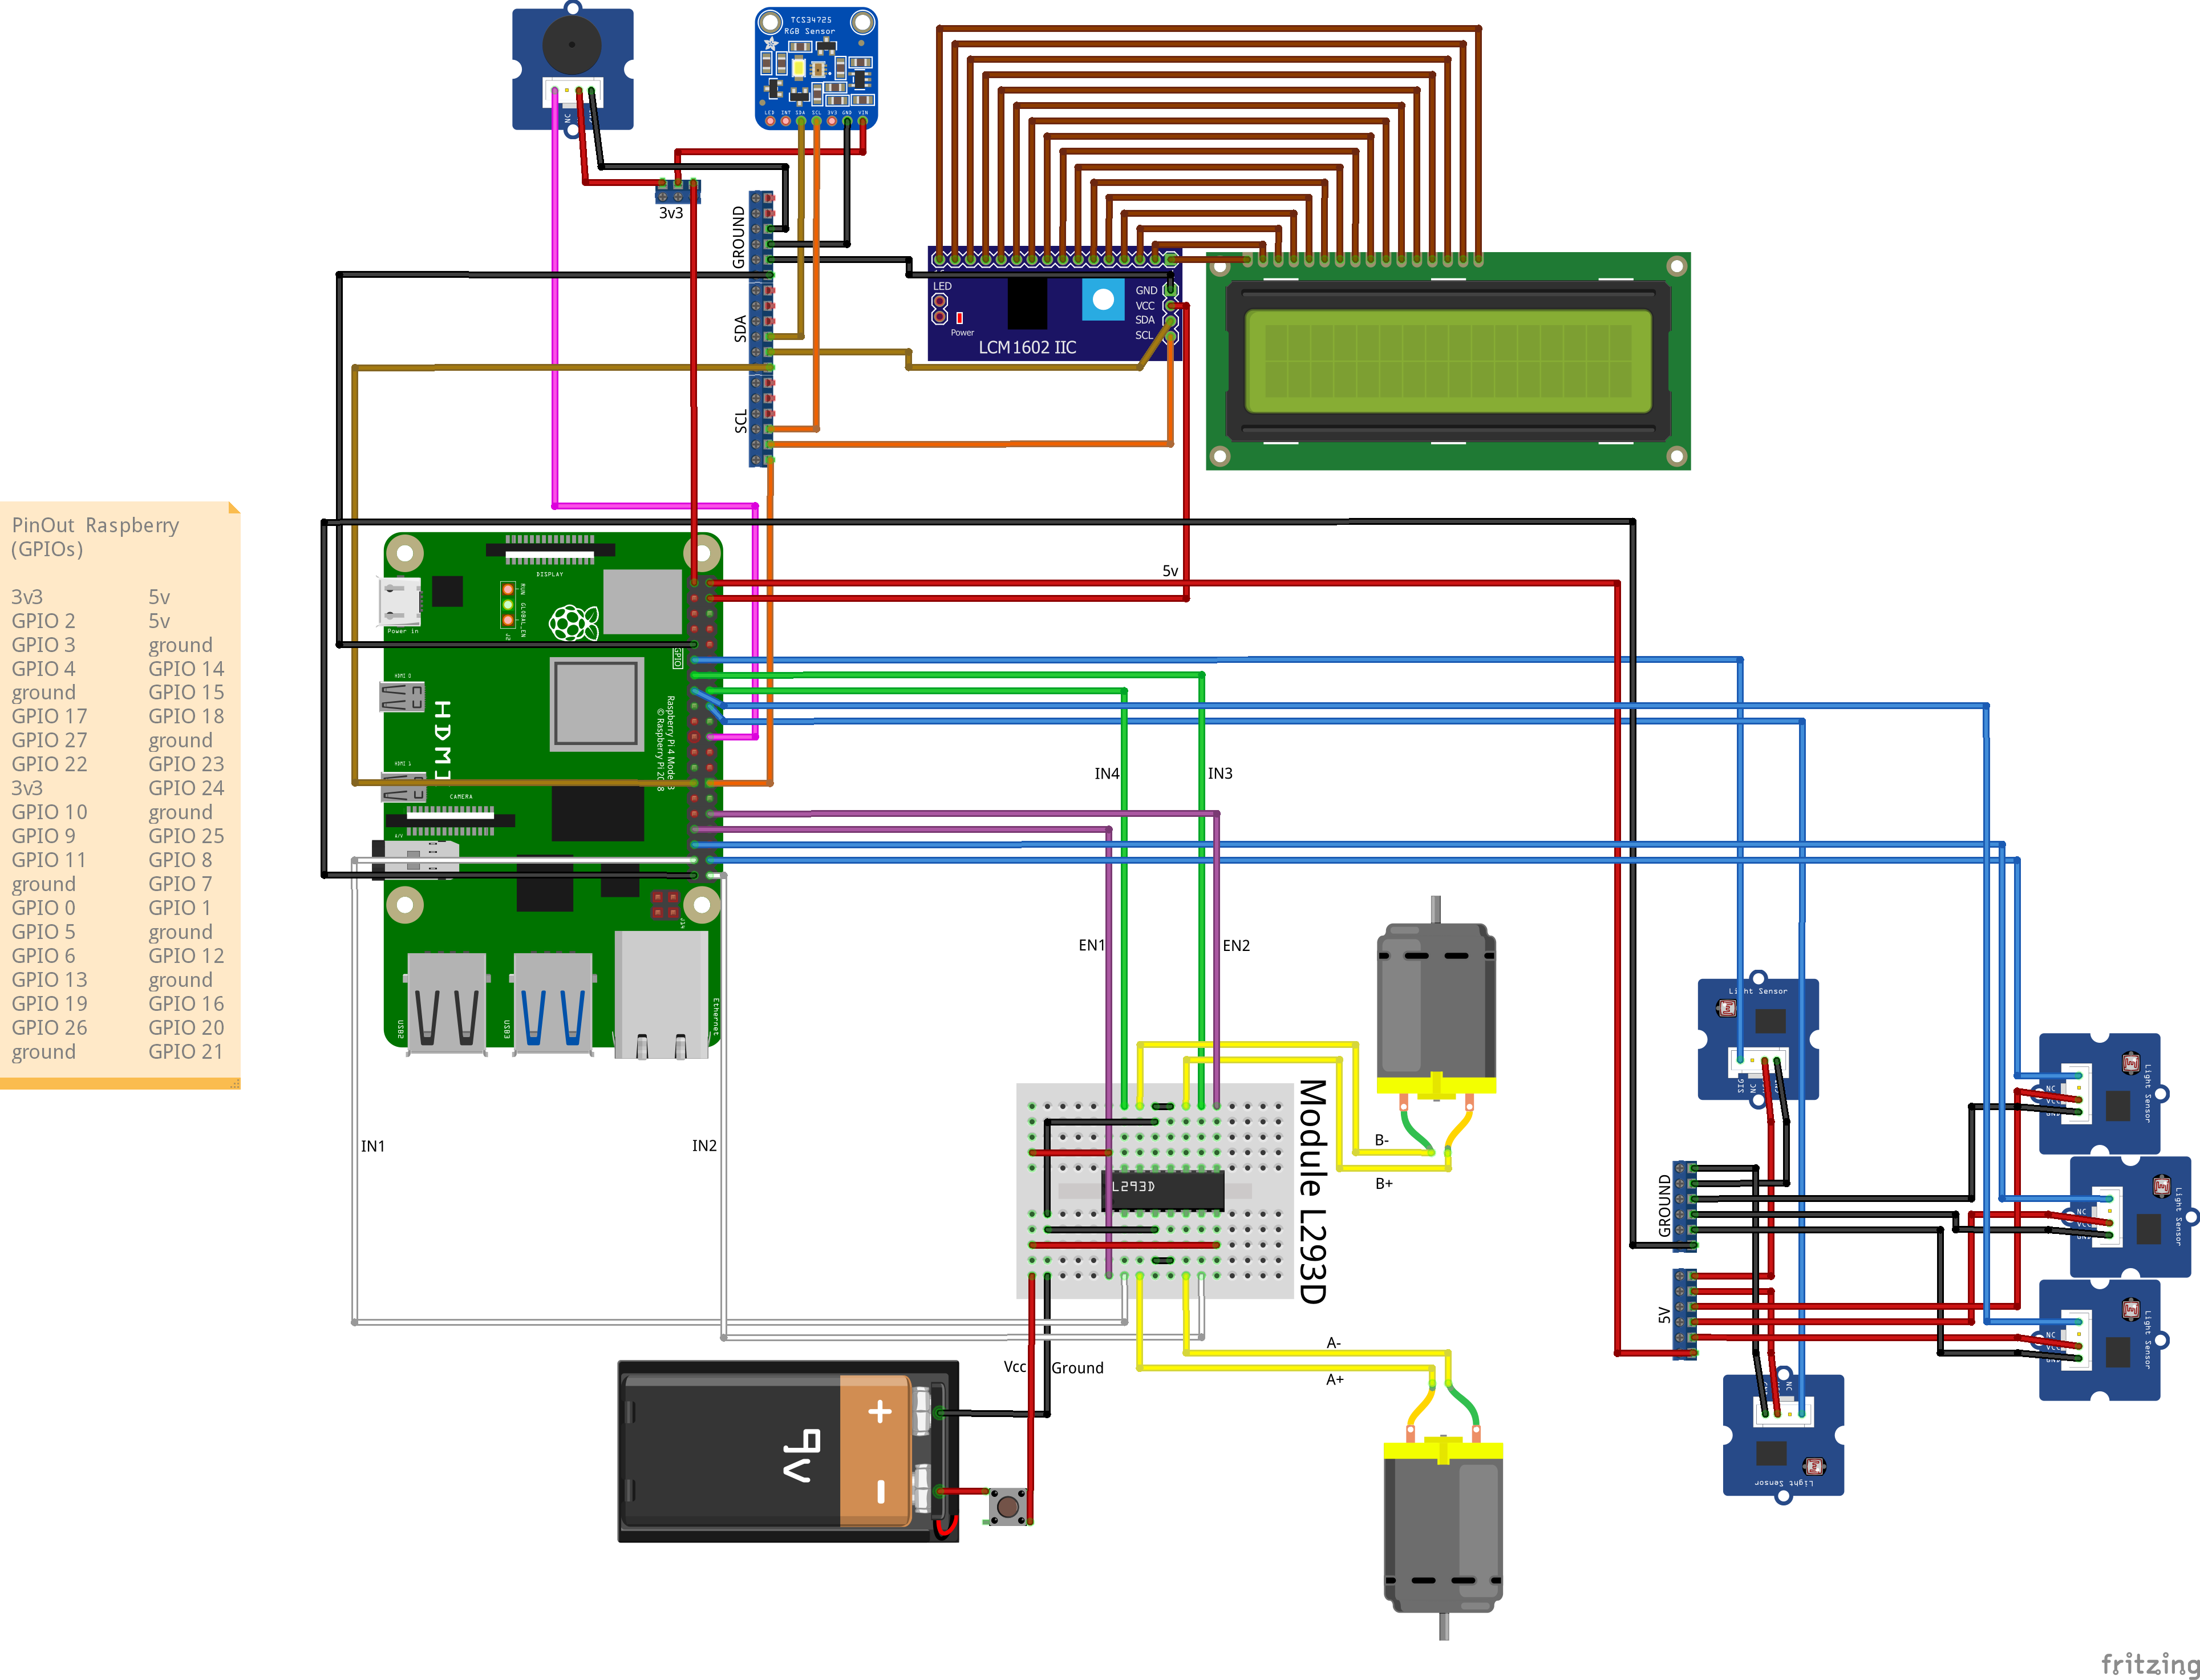
\includegraphics[width=1.0\textwidth]{image/schema_fritzing_bb.png}
    \caption{Schéma de notre montage électrique}
    \label{fig:capteurs}
\end{figure}

Ces schémas ont été réalisés avec le logiciel fourni par l'INSA : \url{https://fritzing.org}

\section{Choix de câblage et choix technique}
Cette section détaille le choix de câblage des différents composants de notre système ainsi que les raisons techniques de ces choix.

La première discussion fut sur la position des capteurs de ligne. Notre première idée était de placer deux capteurs à l'avant de part et d'autre de la ligne ainsi que deux capteurs à l'arrière permettant de détecter les intersections. Après plusieurs tests, nous avons remarqué que les deux roues du robot n'avançaient pas à la même vitesse. Avec seulement deux capteurs à l'avant, le robot n'arrêtait pas d'effectuer des petites corrections vers la droite et vers la gauche, ce qui rendait le suivi de ligne peu efficace et peu stable. Nous avons donc décidé d'utiliser cinq capteurs afin d'assurer un suivi de ligne précis et fiable. Trois capteurs ont été placés à l'avant et deux à l'arrière. Les capteurs avant sont principalement utilisés pour le suivi de la ligne noire. Ils vont permettre au robot de se recentrer sur la ligne en permanence et sont également utilisés pour déterminer le moment où le robot doit s'arrêter de tourner lors des changements de direction. Les deux capteurs à l'arrière sont toujours utilisés pour détecter les intersections.

Les autres composants tel que le LCD, le moteur, le buzzer etc n'ont pas été compliqués à placer car peu importe leurs emplacements sur le robot ils auraient eu la même utilité. 

Le capteur RGB avait été initialement mis en dessous du robot, vers l'arrière. Mais après plusieurs tests, nous avons constaté que cette position entraînait une détection trop tardive de la pastille. C'est pourquoi nous avons décidé de le mettre juste avant la première roue, ce qui a permis d'améliorer sa précision de la détection. 

En revanche, le positionnement des piles n'a pas été si évident. Au départ, nous avions placé les piles à l'intérieur du robot mais après plusieurs essais, nous avons constaté que l'accès était assez compliqué. En effet, en bougeant tous les composants pour mettre les piles, des câbles se détachaient ce qui n'était pas pratique et dangereux. Afin d'améliorer la sécurité, nous avons donc décidé de sortir les piles de l'intérieur et de les positionner sur la partie supérieure avec la batterie. Ce choix permet une meilleure organisation des câbles ce qui réduit les risques électriques et facilite également l'accès aux piles.
Avant d'installer définitivement les composants sur le robot, nous avons effectué des tests individuels afin de bien vérifier le bon fonctionnement de chaque composant.

La figure ci-dessous permet de mieux comprendre la répartition des capteurs sur le robot.

\begin{figure}[H]
    \centering
    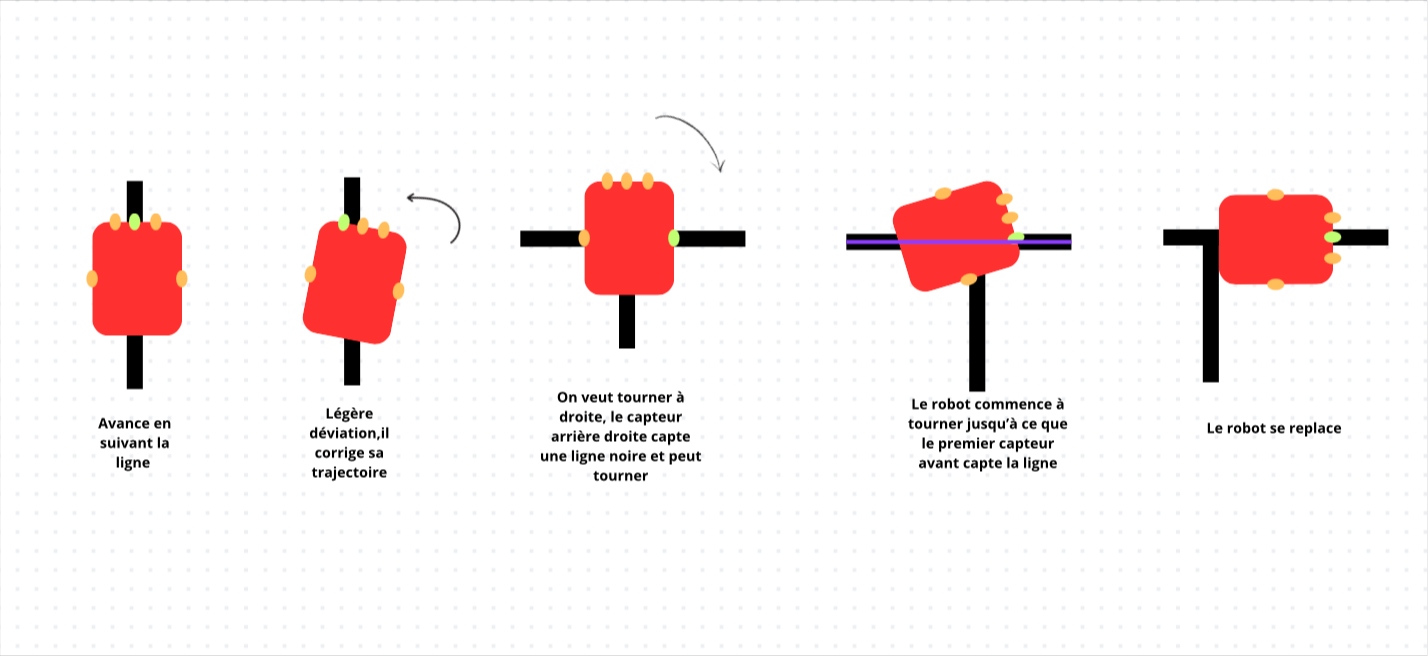
\includegraphics[width=1.0\textwidth]{image/robot_tourne.png}
    \caption{Schéma expliquant la disposition des capteurs de ligne}
    \label{fig:capteurs}
\end{figure}


\subsection{Ecran LCD} 
L'écran LCD communique avec la Raspberry Pi par le protocole I2C. Nous avons donc utilisé :
\begin{itemize}
    \item le GPIO 2 pour la ligne SDA (Data)
    \item le GPIO 3 pour la ligne SCL (Clock)
\end{itemize}
L'écran est alimenté en 5V depuis la Raspberry Pi.

\subsection{Capteur RGB}  
Le capteur RGB fonctionne également avec le protocole de communication I2C. La Raspberry Pi dispose d'un seul couple de GPIO pour SDA et SCL, nous avons donc dû utiliser des dominos afin de brancher à la fois l'écran LCD et le capteur RGB sur les mêmes lignes I2C. Le capteur RGB est cependant lui alimenté en 3.3V.

De même, étant donné le nombre de composants utilisant le 3.3 V et les GND, nous avons utilisé des dominos afin de brancher plusieurs composants à la fois sur les mêmes lignes.

\subsection{Buzzer}
Le buzzer ne nécessite pas de protocole particulier. Nous l'avons donc connecté sur le GPIO 25. Il est alimenté par la Raspberry Pi en 3.3 V également.

\subsection{Capteurs de ligne}
Les capteurs de lignes ont été mis sur des GPIO n'ayant pas de particularité c'est à dire le GPIO (17, 22, 24, 19, et 20). Ce choix permet une lecture simple des signaux numériques. Ils sont tous alimentés en 3.3 V.

\subsection{Moteur}  
Les connexions pour les moteurs ont été choisies de la manière suivante :
\begin{itemize}
    \item EN1 et EN2 sur les GPIO 13 et 12 pour le contrôle en PWM. Ces 2 GPIO permettent de contrôler la vitesse des moteurs.
    \item IN1, IN2, IN3, IN4 ont été mis sur des GPIO standards. Ils nous permettent de définir le sens de rotation des moteurs. (GPIO 26, 21, 27 et 23)
    
\end{itemize}
Cette configuration permet un contrôle indépendant des moteurs et une modulation de la vitesse essentielle pour la navigation précise du robot.

\subsection{Controleur L293D}

La première zone gère les courants nécessaires à la motorisation :
\begin{itemize}
    \item \textbf{A+,A- \& B+ , B- :} Connexion des deux moteurs à courant continu. Le sens de rotation est déterminé par l'ordre des fils
    .
    \item \textbf{VIN / GND :} Reliée aux piles. Le fil positif est relié à la borne VIN et la masse au GND.
\end{itemize}

La deuxième zone assure l'interface avec les ports GPIO de la Raspberry Pi :
\begin{itemize}
    \item \textbf{VCC / GND :} Alimentation logique du module reliée directement aux sorties 5V et GND de la Raspberry Pi.
    \item \textbf{IN1, IN2, IN3, IN4 :} Entrées de commande directionnelle. Reliées sur les GPIO déja cités plus haut.
    \item \textbf{EN1, EN2 :} Ces broches permettent d'activer les moteurs.
\end{itemize}

\section{Bilan de puissance et estimation de l'autonomie}

Cette section présente l'analyse énergétique du robot. L'objectif est de valider l'utilisation de ces composants par rapport à leurs consommations.

\subsection{Méthodologie d'estimation}
N'ayant pas toutes les fiches techniques de chaque composant, nous avons basé notre bilan de puissance sur des standards industriels et les documentations en ligne des composants équivalents. 

\begin{itemize}
    \item \textbf{Raspberry Pi 4 :} La documentation officielle [1] indique une consommation de \textbf{540 mA} au repos (Idle). Cependant, nous avons retenu une valeur de \textbf{600 mA} pour nos calculs. Cette différence de 60 mA permet de prendre en compte l'activité processeur lors de l'exécution de notre code et de gestion des capteurs, qui sollicite davantage les ressources que le mode repos.
    
    \item \textbf{Moteurs :} Pour les moteurs, plusieurs sources [2] indiquent un courant à vide de 200 mA. Nous avons choisi d'utiliser la valeur de \textbf{400 mA} par moteur. Nous avons augmenté le courant car à vide il ne prend pas le poids du châssis et n'a pas la contrainte du frottement du sol.
    
    \item \textbf{Contrôleur L293D :} La datasheet de Texas Instruments [3] indique un courant de repos logique (Vss) typique de 24 mA à 30 mA. Nous avons pris cette valeur à \textbf{30 mA}.
\end{itemize}

Nous avons appliqué cette approche de sur-estimation volontaire pour garantir que l'autonomie finale du robot soit une valeur minimale garantie, même en cas de forte sollicitation des moteurs ou du processeur.

\subsection{Tableau récapitulatif des consommations}

Afin de garantir la précision du système, nous avons opté pour une séparation entre le \textbf{Circuit de Logique} et le \textbf{Circuit d'Actionnement}. Cette distinction est importante car la Raspberry Pi et les capteurs nécessitent une tension constante de 5V. En isolant ce circuit sur une batterie dédiée, nous évitons les chutes de tension brusques provoquées par le démarrage des moteurs, qui pourraient entraîner un plantage du système d'exploitation.En séparant physiquement leur alimentation de celle des composants de calcul, nous limitons la propagation de bruits électriques sur les bus de communication (notamment l'I2C utilisé pour le capteur couleur et l'écran LCD), assurant ainsi une lecture fiable des données capteurs.

\begin{table}[h!]
\centering
\begin{tabular}{@{}llll@{}}
\toprule
\textbf{Composant} & \textbf{Tension} & \textbf{Courant ($I$)} & \textbf{Source de la donnée} \\ \midrule
\textit{Circuit Logique} & \textbf{5.0 V} & & \\
Raspberry Pi 4 & 5.0 V & 600 mA & Documentation RPi [1] \\
Écran LCD 1602 (I2C) & 5.0 V & 26 mA & Wiki Waveshare [4] \\
Capteur RGB (TCS34725) & 3.3 V & 15 mA & Datasheet ams OSRAM [5] \\
Capteurs de ligne (x5) & 3.3 V & 50 mA & Valeur standard (10mA/u) \\
\textbf{Total} & & \textbf{691 mA} & \\ \midrule
\textit{Circuit Actionnement} & \textbf{7.4 V} & & \\
2x Moteurs CC (en charge) & 7.4 V & 800 mA & Datasheet TT Motor [2] \\
Controleur L293D & 5.0 V & 30 mA & Datasheet TI [3] \\
\textbf{Total} & & \textbf{830 mA} & \\ \bottomrule
\end{tabular}
\caption{Synthèse des consommations électriques}
\end{table}

\subsection{Estimation de l'autonomie théorique}

L'autonomie est calculée par la formule : $Autonomie = \frac{C_{batt}}{I_{conso}}$.

\textbf{Partie Logique (Batterie USB de 10 000 mAh ( valeur trouvée sur la batterie elle même) :}
\begin{equation}
Autonomie_{Logique} = \frac{10 000 \text{ mAh}}{691 \text{ mA}} \approx 14, 4 \text{ heures}
\end{equation}

\textbf{Partie Actionnement :}
\begin{equation}
Autonomie_{Actionnement} = \frac{2500 \text{ mAh}}{830 \text{ mA}} \approx 3,0 \text{ heures}
\end{equation}

L'autonomie est donc largement suffisante pour les phases de tests et la compétition.

Ces valeurs nous semblent cohérentes avec nos essais en séance de TP. En effet, nous n'avons rechargé notre batterie qu'une ou deux fois sur l'ensemble du projet car elle ne s'était jamais réellement vidée. La valeur de 3h pour l'actionnement est cohérente également car elle correspond à une utilisation à plein régime et en continu. Lors des différents tests, nous n'avons jamais réalisé des sessions aussi longues sans interruption. Cependant, nous avons remarqué qu'au bout de quelques heures, le robot pouvait avancer légèrement moins vite. Ce phénomène s'explique par la baisse progressive de la tension nominale des piles NiMH lors de leur décharge, ce qui réduit directement la puissance fournie aux moteurs.

\section{Rôles des composants}

\subsection{Raspberry Pi}
La Raspberry Pi est comme le cerveau du robot, elle exécute les programmes pour contrôler les moteurs et elle interprète les données des capteurs.

\subsection{Batterie USB-C}
Cette batterie permet d'alimenter la Raspberry Pi. Cette batterie permet d'assurer que la Raspberry Pi reste toujours allumée même si les moteurs sont éteints.

\subsection{Pile}
Les piles vont fournir un courant plus élevé aux moteurs, ces piles sont nécessaires pour transmettre un courant assez élevé aux moteurs sans surcharger la Raspberry Pi.

\subsection{Ecran LCD} 
Le rôle de l'écran LCD est d'assurer l'interface homme-machine du robot. Il affiche en temps réel les informations suivantes : les ordres exécutés (AV, TG, TD), la couleur détectée par le capteur RGB ainsi que l'état du robot (initialisation, arrêt).
L'écran LCD est un afficheur utilisé par le protocole de communication I2C et à partir d'un module d'extension ( PCF8574) il va nous faciliter les branchements.
Le protocole I2C permet de réduire le nombre de fils nécessaires en utilisant seulement : SDA (données) et SCL (clock).

\subsection{Capteur RGB}
Le capteur RGB permet au robot de détecter la couleur des pastilles présentes sur le circuit. Au départ il devra détecter une pastille rouge puis il devra détecter les pastilles vertes qui seront les points de passage obligatoire, et pour finir il devra revenir à la pastille rouge. Lorsqu'une de ces couleurs est détectée, le robot doit afficher cette information sur l'écran LCD et activer le buzzer.
Ce capteur mesure donc l'intensité de la lumière réfléchie par trois composantes qui sont les trois couleurs primaires, le rouge , le vert et le bleu. Une LED est intégrée à ce module et permet d'éclairer la surface à analyser. Des photodiodes internes mesurent la lumière réfléchie et le capteur convertit ces mesures en valeurs numériques. Ces valeurs sont transmises vers la Raspberry Pi via le protocole bus I2C. 
Le programme devra donc comparer les valeurs R, G, B afin de déterminer la couleur dominante détectée.

\subsection{Buzzer}
Le buzzer va permettre d'émettre un bip lorsque le robot atteint un point de passage obligatoire, c'est à dire lorsque le capteur RGB a détecté une pastille rouge ou verte.
Le buzzer est commandé directement par une sortie GPIO de la Raspberry Pi. Lorsque la broche GPIO est mise à l'état haut le buzzer est alimenté et produira en conséquence un son. 

\subsection{Capteurs de ligne }
Les capteurs de ligne permettent au robot de suivre les lignes noires tracées sur le sol et de détecter les croisements. Ils sont indispensables pour assurer le guidage précis du robot dans la ville.
Chaque capteur fonctionne à l'aide d'une LED infrarouge et d'un phototransistor. Une surface claire réfléchit fortement la lumière alors qu'une ligne sombre va absorber cette lumière. Selon cette quantité de lumière reçue, le capteur fournira un signal logique (0 ou 1) à la Raspberry Pi. 

\subsection{Moteurs}
Les moteurs assurent les déplacements du robot : avancer en ligne droite, tourner à gauche, tourner à droite et s'arrêter.
Le robot utilise deux moteurs à courant continu, un pour chaque roue. Nous allons pouvoir contrôler le sens et la vitesse de chaque moteur via PWM.

\subsection{Interrupteur}
L'interrupteur va nous permettre de couper ou de remettre l'alimentation électrique des moteurs sans affecter la Raspberry Pi. Ce composant va permettre de mettre le robot en sécurité avant l'intervention, de démarrer ou d'arrêter le déplacement du robot facilement et de préserver la Raspberry Pi lorsqu'on manipule le robot.

\subsection{Contrôleur L293D}
Le contrôleur L293D sert d'interrupteur automatique : il reçoit de petits signaux de la Raspberry Pi pour laisser passer la forte puissance de la batterie vers les moteurs, ce qui va permettre ainsi de contrôler leur direction et leur vitesse sans griller la carte.

\section{Organigramme}

Nous avons réalisé plusieurs sous programmes afin de répondre aux problèmes. 
L'analyse descendante étant assez grande, nous l'avons divisé en trois pour mieux la voir. Mais si vous souhaitez la consulter entièrement vous pouvez aller sur le lien suivant :
\href{https://www.canva.com/design/DAG614fXwmo/bapIBcVTE0LtQyUYekXYlA/edit?utm_content=DAG614fXwmo&utm_campaign=designshare&utm_medium=link2&utm_source=sharebutton}{Analyse Descendante complète}.

La première partie contient les fonctions basiques : 

\begin{figure}[H]
    \centering
    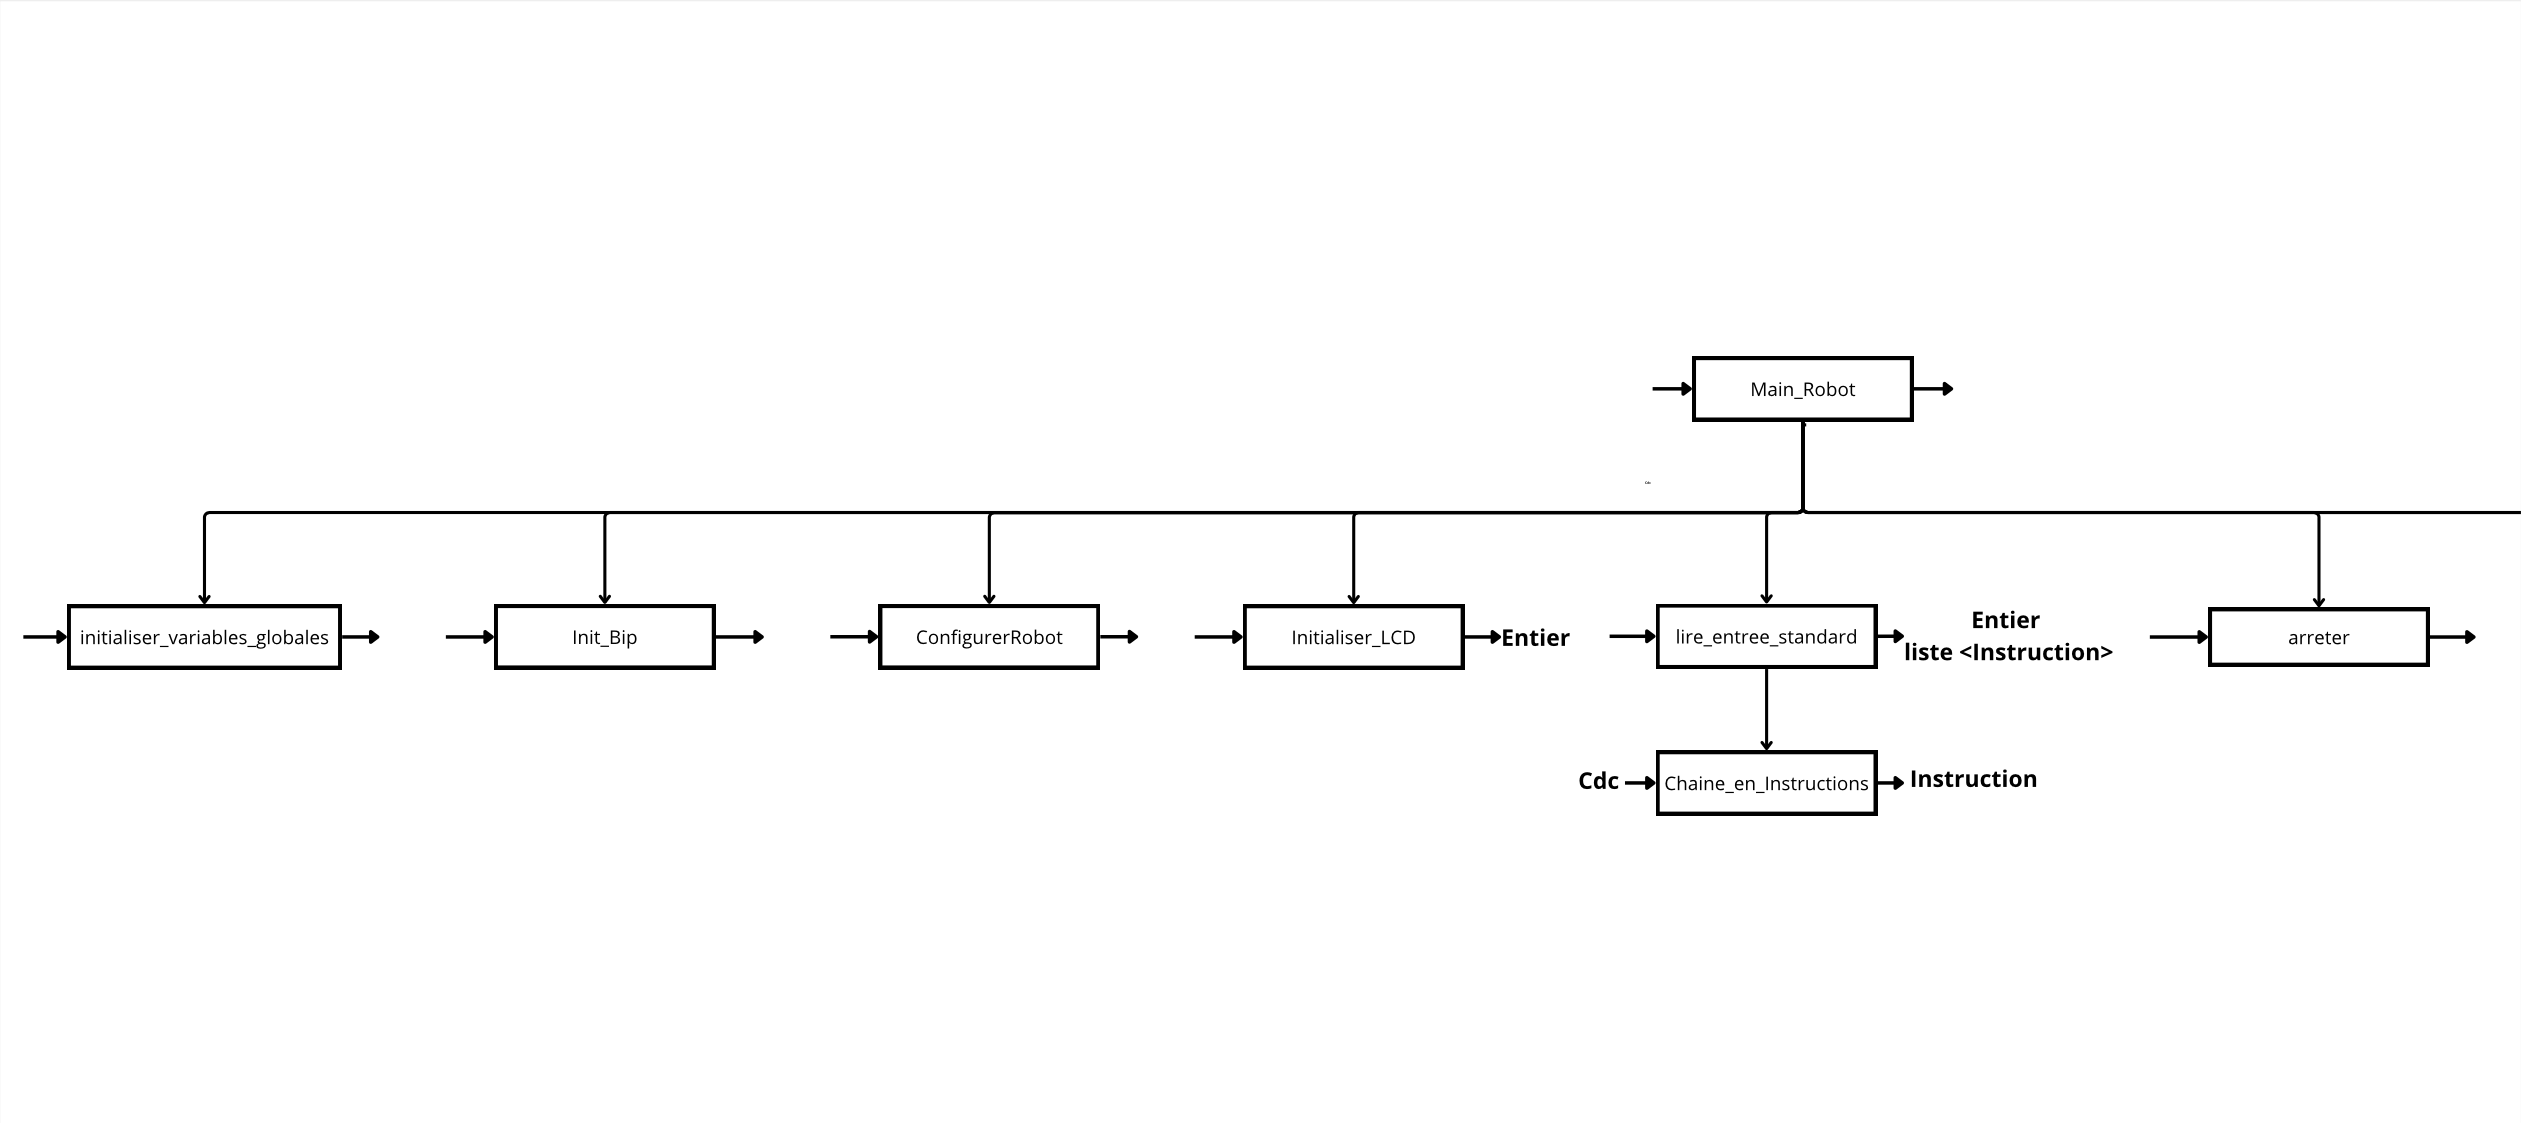
\includegraphics[width=1.0\textwidth]{image/Analyse_Robot_1.png}
    \caption{Première partie de l'analyse descendante}
    \label{fig:capteurs}
\end{figure}

La seconde partie représente la procédure déplacer qui est utilisé par le main.

\begin{figure}[H]
    \centering
    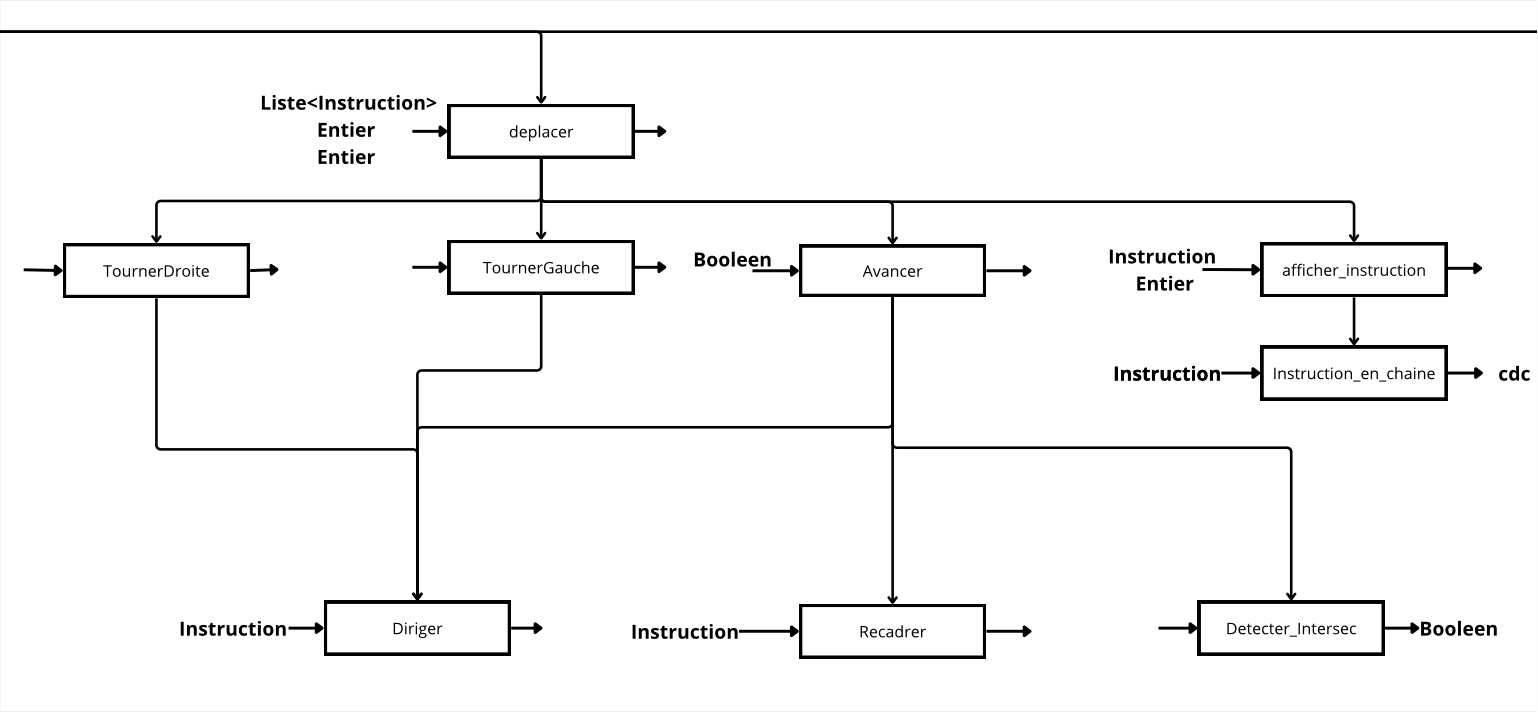
\includegraphics[width=1.0\textwidth]{image/Analyse_Robot_2.png}
    \caption{Seconde partie de l'analyse descendante}
    \label{fig:capteurs}
\end{figure}

La dernière partie représente le thread\_detection\_pastille qui est initialisé dans le main également.

\begin{figure}[H]
    \centering
    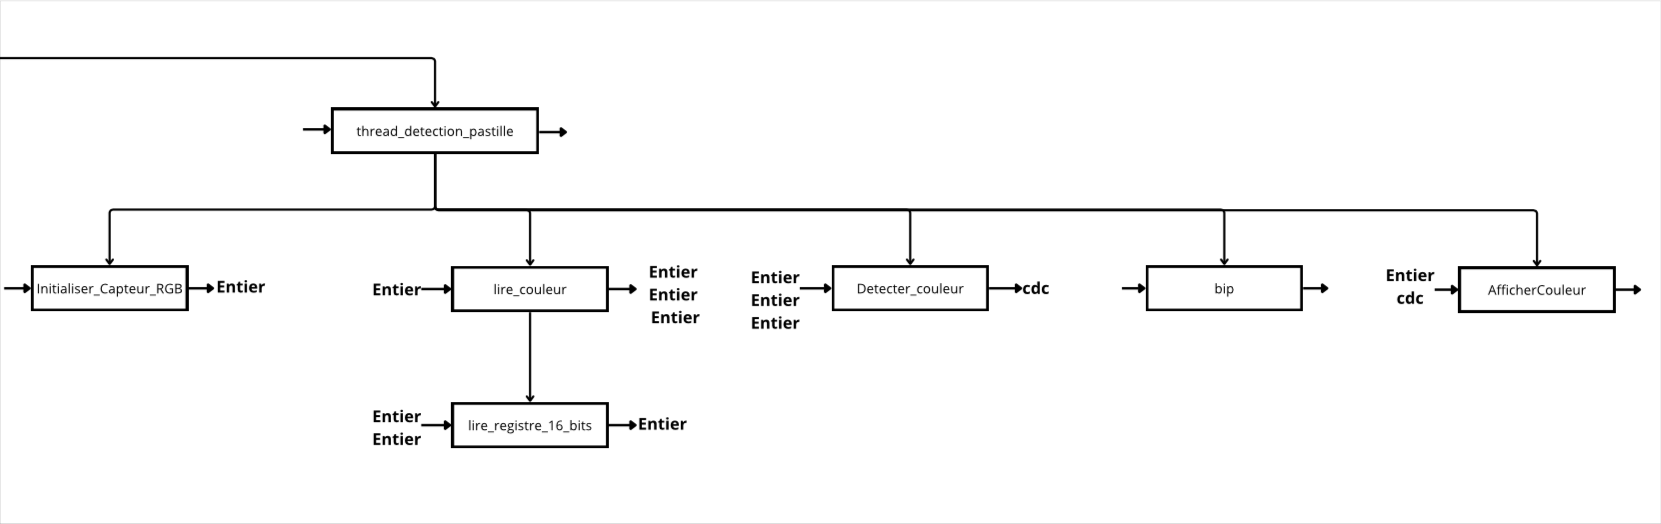
\includegraphics[width=1.0\textwidth]{image/Analyse_Robot_3.png}
    \caption{Dernière partie de l'analyse descendante}
    \label{fig:capteurs}
\end{figure}

\begin{description}

\item[\textbf{main}] : permet d'utiliser l'ensemble du système et de piloter le déroulement global du programme du robot. Il configure toutes les broches, initialise les variables globales utilisées par le programme. Nous avons décidé d'utiliser un thread pour la détection des pastilles de couleur car gérer la détection de ligne et de pastilles dans le même processus était trop compliqué, il entraînait des délais d'exécution. Ces délais provoquaient des erreurs de trajectoire et le robot se perdait rapidement.Le thread permet donc d'exécuter la détection de couleur en parallèle du déplacement du robot. Le main initialise donc ce thread. Ensuite il lit les instructions de déplacement sur l'entrée standard et réalise le parcours en entrée grâce à la procédure déplacer. Une fois le parcours terminé, le main arrête proprement le thread de détection de pastille et libère les ressources partagées.

\item[\textbf{configurerRobot}] : permet d'initialiser l'environnement matériel du robot. On initialise la bibliothèque wiringPi, configure les broches des différents capteur et du moteur.

\item[\textbf{InitialiserLCD}]: permet d'initialiser l'écran LCD.

\item[\textbf{init\_Bip}]: permet d'initaliser le buzzer.

\item[\textbf{Initialiser\_variables\_globales}]: permet d'initialiser les variables globales liées au fonctionnement multithread du programme. Elle initialise le mutex qui est utilisé pour protéger l'accès aux données partagées entre le thread principal et celui de la détection de pastille.

\item[\textbf{lire\_entree\_standard}] : permet de récupérer les instructions saisies dans le terminal en entrée standard.

\item[\textbf{arreter}]: permet d'arrêter le robot.

\item[\textbf{Chaine\_en\_Instructions}]: permet de transformer les chaînes de caractère lue en entrée standard et de les transformer en Instruction.

\item[\textbf{deplacer}]: permet d'effectuer le déplacement complet du robot, cette procédure vérifie si une pastille n'a pas été détectée. Cette procédure assure la coordination entre l'affichage sur le LCD, la détection de pastilles et le déplacement du robot.

\item[\textbf{detecter\_Intersec}] : regarde si un des capteurs de derrière détecte une intersection.

\item[\textbf{tourner\_gauche et tourner\_droite }]: font tourner le robot à gauche ou droite jusqu'à ce que un des capteurs de devant détecte la ligne noire. 

\item[\textbf{diriger}]: reçoit une instruction de déplacement ( AV,TG ...) et configure les moteurs en conséquence en ajustant la vitesse et le sens de rotation.

\item[\textbf{recadrer}]: lorsque le robot s'écarte légèrement de sa trajectoire, cette procédure ajuste la vitesse relative des moteurs pour le remettre sur la bonne ligne.  Elle agit comme un correcteur pour stabiliser le déplacement.

\item[\textbf{avancer}] : fait avancer le robot tout en surveillant la trajectoire grâce aux capteurs de ligne. Si le robot détecte un écart il se recadre automatiquement. Lorsque la pastille de fin rouge est détectée, la fonction arrête le robot.

\item[\textbf{afficher\_instruction}]: permet d'afficher une instruction sur le LCD.

\item[\textbf{Instruction\_en\_chaine}]: transforme une instruction en chaîne de caractère.  

\item[\textbf{thread\_detection\_pastille}]: Cette fonction est exécutée dans un thread séparé et surveille en permanence les capteurs de couleur pour détecter les pastilles sur le parcours. Lorsqu’une pastille est détectée, elle met à jour des variables globales partagées, protégées par un mutex, afin que le thread principal puisse ajuster le déplacement du robot ou l’arrêter si nécessaire.

\item[\textbf{initialiser\_capteur\_RGB}]: Initialise le capteur RGB.

\item[\textbf{AfficherCouleur}]: affiche la couleur de la pastille sur le LCD.

\item[\textbf{Detecter\_couleur}]: à partir des valeurs de R G et B il détermine s'il s'agit de vert ou de rouge. ( les autres cas ne sont pas pris en compte).

\item[\textbf{Bip}]: déclenche le buzzer pendant un certain temps.

\item[\textbf{lire\_couleur}]: lis les couleurs du capteur RGB, c'est à dire il donne une valeur que le capteur capte pour les trois couleurs primaires.

\item[\textbf{lire\_registre\_16\_bits}]: utilisé pour lire des registre de 16 bits. Très utile pour l'utilisation du LCD.


\end{description}

\section{Difficultés rencontrées et pistes d'améliorations}

Le premier problème que nous avons rencontré est apparu lors des premiers tests des moteurs. En effet, nous avions connecté le IN1 sur le GPIO 4, cependant ce GPIO a une double fonction qui est la clock. La roue qui était donc controlée par ce GPIO tournait par intermittence. Ce problème a donc été réglé en changeant le IN1 de pin sur la Raspberry, en le mettant sur un GPIO sans fonction particulière.

Après avoir résolu ce problème de GPIO 4, nous avons remarqué que nos deux roues ne roulaient pas du tout à la même vitesse alors qu'elles étaient censées fonctionner de manière identique. Une première solution était de contrôler la vitesse de chacune des roues par PWM mais nous avons préféré remplacer un des moteurs. Même après ce changement, les deux roues n'allaient pas à la même vitesse mais l'écart était moins important nous avons donc conservé cette configuration.

Nous avons également rencontré plusieurs difficultés avec le capteur RGB. En fonction de l'emplacement de la salle où on le faisait, de l'heure de la journée les valeurs des composantes R G et B variaient fortement. En effet , la luminosité avait un impact significatif sur nos valeurs. Dans notre code initial, les conditions de détection des couleurs étaient trop précises sur ces valeurs ce qui n'était pas du tout efficace. Nous avons donc modifié notre code afin de mettre des conditions plus large qui nous a permis de bien détecter la couleur de la pastille.

Enfin,tout au long du projet, nous avons procédé à de nombreux tests et ajustements. Cette démarche itérative a permis de corriger progressivement les erreurs et d'améliorer la fiabilité globale du robot. 